% ------------------------------------------------------------------------
% -*-TeX-*- -*-Hard-*- Smart Wrapping
% ------------------------------------------------------------------------
\def\baselinestretch{1}

\chapter{Methodology Design}

\def\baselinestretch{1.44}

%%% ----------------------------------------------------------------------

This chapter describes the overall methodology design for my dissertation project, which include web portal design, chatbot design, and community forum design. 
   
\smallskip

%%% ----------------------------------------------------------------------
\goodbreak
\section{Web Portal}
The web portal have a base page as a homepage, then it connects to the other pages. User can be navigate through all the pages easily. The client side of the web application is developed using HTML, CSS, Bootstrap, Javascript, and Django framework. 

\subsection{Architectural Design}
The architecture of a website refers to the pages of the website organised in a hierarchical fashion. The internal connecting displays this structure in a clear and concise manner. Users of your website should be able to readily access the information they need, and the structure of your website should also assist search engine crawlers comprehend the connection between the various pages \citep{web}. You may improve the user experience of your website by designing it using a structure that has been used on the website. Even if you have the most excellent content in the world, visitors won't stick around if they can't locate what they're looking for on your website. The home page serves as the starting point for the structure of most websites, which takes the form of a rooted tree graph. The pages that have links leading out from the homepage are referred to as branches, and from that point forward, each page has further branches growing out of it. These branches ultimately connect to one another. 

Figure \ref{fig:4} illustrates the architectural design of the web portal. The website architecture here is very simple. The landing page is the homepage, which will hold all the summary information and the AI chatbot. AI chatbot will remain on the same position on the web portal all the time. From homepage other pages can be accessed by the navigation menu, description links, and html sitemap on footer. All the page will be simple and user can be moved back to homepage from any page. The linked pages includes:
\begin{enumerate}[label=\arabic*.]
	\item \textbf{About Dementia:} This page highlights the information and knowledge about dementia.
	\item \textbf{Dementia Learning:} This page displays the detailed learning for the dementia care.
	\item \textbf{Technologies in Dementia:} This page holds information regarding technological solutions for the dementia care.
	\item \textbf{Research \& News:} This page lists recent research and news regarding dementia.
	\item \textbf{Community Forum:} This page is the homepage of the community forum.
\end{enumerate}

\begin{figure}[!h]
	\centering
	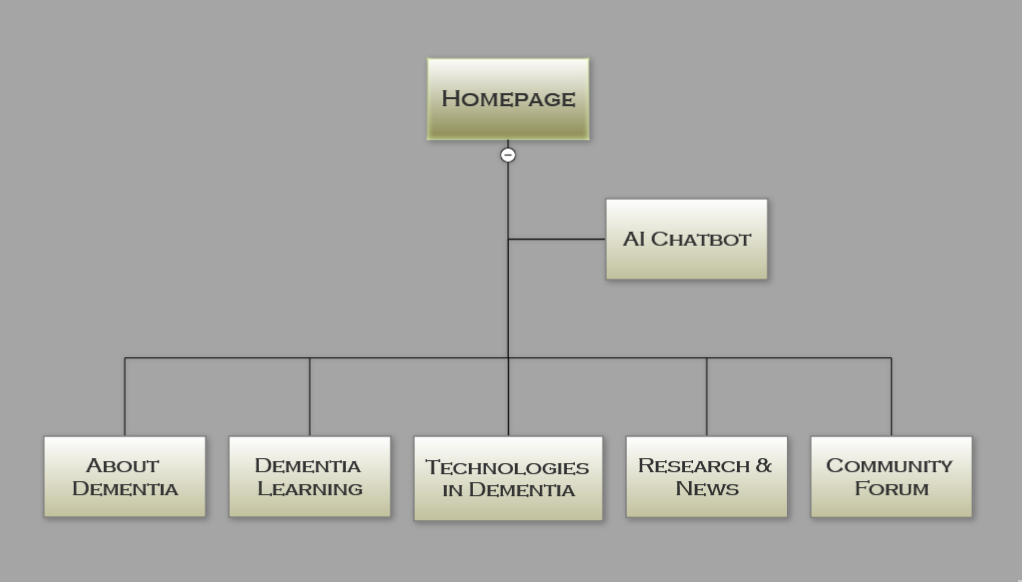
\includegraphics[width=\linewidth]{arch_design}
	\caption{Architectural design of the web portal.}
	\label{fig:4}
\end{figure}

\section{Chatbot}
The functionality of retrieval-based bots of an AI chatbot is built on the idea of oriented patterns or graphs. The bot is programmed to choose which of a limited number of prepared replies is the most appropriate to rank as the best response. The replies that are shown here are either keyed in by hand or are derived from a knowledge base that contains information that already exists. The client side of the chatbot is developed using HTML, CSS, Javascript, and Flask framework.

\subsection{Chatbot Concept}
The data is necessary for training my deep learning-based model, which I want to construct. However, given that this is a chatbot devoted to the subject of dementia, I will not be collecting or downloading any massive dataset. To train the model, I need just generate my own dataset. In order to make this datasets, I need to know exactly which intents I will be teaching. The "intent" of a user's interaction with a chatbot, or the motivation behind a user's communication to the chatbot, is what is meant by the term "intent." These intentions may differ from one chatbot solution to the next, depending on the domain for which I am creating the solution. Therefore, it is crucial that I learn the appropriate chatbot intentions as they pertain to the domain with which I will be interacting.

Understanding what users say or want to do is crucial for the chatbot's ability to respond appropriately, whether that's with a solution to a query, a search in a topic knowledge base, or any number of other activities. That's why it's crucial for the chatbot to read between the lines of user communications (to determine what the user means). The plan is to first determine the various intents that will be used, then create training data for those intents, and then train the chatbot model using the data from those training samples as model training data (X) and the intents themselves as model training categories (Y).

\subsubsection{Natural Language Toolkit (NLTK)}
With Python, NLTK is the go-to framework for manipulating human language data. Easy-to-use interfaces to more than 50 corpora and lexical resources like WordNet are included, as well as a set of text processing libraries for tasks like tokenization, classification, parsing, tagging, stemming, and semantic reasoning, as well as wrappers for commercial-grade NLP libraries and a lively community forum.

\subsubsection{TF-IDF}
Each document's TF-IDF (Term Frequency-Inverse Document Frequency) vectors will be calculated. This will produce a matrix in which each column has a different term from the introductory lexicon. The TF-IDF formula is the standard statistical approach for determining a word's importance inside a text. 

Phrase frequency, sometimes known as TF, refers to the number of times a certain term occurs in a particular text. IDF, which stands for "inverse document frequency," is a metric that determines the importance of a word inside a document by determining whether or not the word is used often across the whole text. According to the rationale behind the TF-IDF algorithm, the words that are used often in a text are less significant than the ones that are used seldom. The good news is that scikit-learn provides you with an in-built TfIdfVectorizer class that makes it very simple to generate the TF-IDF matrix.

\subsubsection{Cosine Similarity}
After obtaining the matrix, it is now simple for me to determine a score for the degree of resemblance. There are a few other approaches that may be used to do this, such as the Euclidean, Pearson, and cosine similarity scores. Once more the, there is no correct response to the question of which result is the best. I will be calculating a numerical amount that represents the similarities of the two words by using the cosine similarity, which is a statistical method. It is possible to make use of the cosine similarity score due to the fact that it is not reliant on the magnitude and may be calculated in a reasonably short amount of time (particularly when the scores of TF and IDF are taken into consideration).

\subsection{Workflow Diagram}
A step-by-step, linear depiction of a workflow from the beginning to the end is what is known as a workflow diagram. It illustrates how certain responsibilities, activities, or resources are distributed across several individuals or organisations. It also demonstrates the steps that need to be taken by your team in order to complete a job.

\begin{figure}[!h]
	\centering
	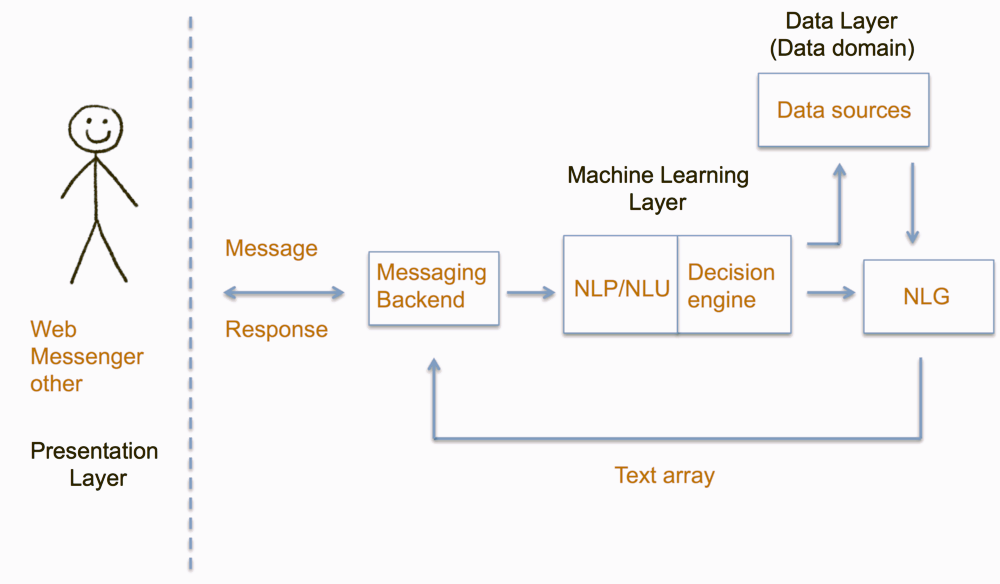
\includegraphics[width=\linewidth]{chatbot}
	\caption{Workflow diagram of the chatbot.}
	\label{fig:5}
\end{figure}

Figure \ref{fig:5} highlights the workflow of the intelligent chatbot. Here,
\begin{enumerate}[label=\arabic*)]
	\item The user poses inquiries to the chatbot, which are subsequently sent to the communication backend via the chatbot.
	\item Implementing natural language processing (also known as what occurs when computers understand language). Because NLP algorithms transform text into structured data, the computer must first translate such simple text request into instructions that it can understand.
	\item At this point, the chatbot will put this information into a decision engine, also known as a trained model, since, in the chatbot's head, it believes that it must fulfil a set of criteria in order to leave the conversational loop.
	\item The use of NLG, which refers to what takes place when computers compose language. NLG procedures take structured data and transform it into text, which is then returned to the user in a form that they can comprehend and relate to.
	\item This collection of user replies is sent back into the messaging backend, where it is processed and then delivered to the user in the form of a response.
\end{enumerate}

\section{Forum}
A community or discussion forum is an online gathering area where individuals may debate, exchange information, and chat to one other about a broad variety of things that they could be engaged in. HTML, CSS, Bootstrap, Javascript, and the Django framework are used to construct the client side of the group discussion forum. SQLite is the underlying technology for the database. 

The administrator is the one who is informed whenever an end-user submits an inquiry with the intention of obtaining information. The doubts subjects may be posted by any user, and any user can respond to the doubts of other users. There is one database in which all of the information is maintained, and that database is centralised. The user is able to post queries and invite other users to participate in Discussion. The database may be updated, but only the administrator has access to do so. This is great for a small workplace, school, or department, or really any organisation that is interested in successfully organising their space. There is a third kind of user known as a connected user who functions as an intermediate user and who, if they have the information, may also provide answers to queries posed by end users. Ability to publish articles and share resources, both of which may be read by users who have registered for the site. The end-user is responsible for making any necessary adjustments or updates whenever fresh data becomes available.

\subsection{Forum Modules}
The community forum includes six main modules, that made the interaction easier and users posts can be seen by everyone.
\begin{enumerate}[label=$\bullet$]
	\item \textbf{Category Module:} This is the primary section, where users may submit their inquiries by choosing a suitable category. Various users may provide responses to their inquiries.
	\item \textbf{Post Question Module:} This section is primarily for those who have already registered. The user is required to register in order for the Administrator to determine who is responsible for posting the questions. These registered people are the only ones who may submit a question in such a thorough way.
	\item \textbf{Registration Module:} The freshly entered user's information may be seen in more depth with the assistance of this module.
	\item \textbf{Comment Module:} Each and every question that is asked will receive an accurate response from the discussion forum staff, and in addition to that, they may get a lot of responses from a variety of different users.
	\item \textbf{Discover Module:} Here, visitors may respond to polls and quizzes. This module is useful for both registered and non-registered users. They may also check out the site for answers.
	\item \textbf{Search Module:} Users may enter their inquiries into this module, and the system will provide relevant results. Articles and innovations containing the search term are linked to in the results. Anyone, registered or not, may do a search.
\end{enumerate}

\subsection{Activity Diagram}
The activity diagram is crucial UML diagram for describing the system's state and behaviour across time. An activity diagram is a kind of flowchart that shows how one task leads to another. This is a system operation, therefore we may call it such. The direction of the flowchart is shown graphically, from one process to the next. This progression may be linear, branching, or concurrent. Using symbols like forks, joins, and others, activity diagrams may represent any kind of branching or branch-and-boundary relationships between two or more flows. Figure \ref{fig:6} shows the activity diagram for the community forum.

\begin{figure}
	\centering
	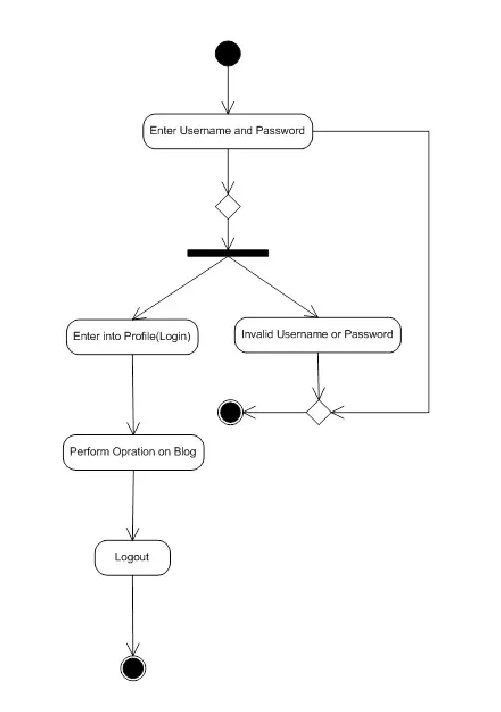
\includegraphics[width=\textwidth]{activity}
	\caption{Activity diagram of the community forum.}
	\label{fig:6}
\end{figure}

\subsection{Use Case Diagram}
Use case diagrams, which are more often known as behaviour diagrams, are used to represent a collection of activities (use cases) that some system or systems (the topic) should or can do in conjunction with one or more users who are not internal to the system (actors). Every use case has to provide some measurable and actionable outcome to the system's actors and other stakeholders in order to be considered successful. Figure \ref{fig:7} illustrates the use case diagram of the community forum.

\begin{figure}[!h]
	\centering
	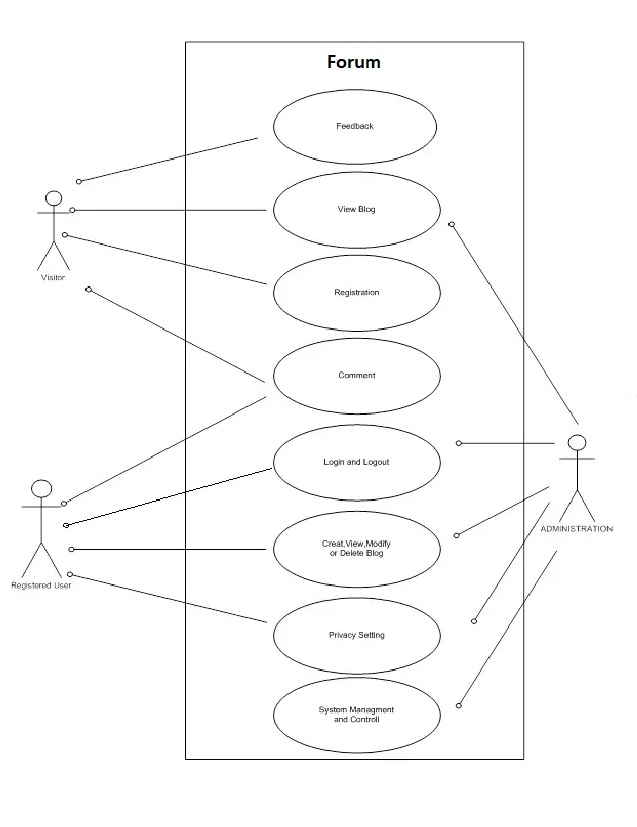
\includegraphics[width=0.8\linewidth]{usecase}
	\caption{Use case diagram of the community forum.}
	\label{fig:7}
\end{figure}

\subsection{Database Design}
Any programme that is designed absolutely needs a database architecture, but data store projects need it much more than other applications. Here, in the forum includes storing the information in the table according to authors, posts, categories, comments, and replies; it is essential that the table be managed in the appropriate manner. The login table for this forum is intended to be one of a kind in that it will only take one username at a time, and both the username and the password should have a length that is larger than zero. Figure \ref{fig:8} shows the database structure design for the forum that includes comprehensive listing of all of the tables and the fields.

\begin{figure}[!h]
	\centering
	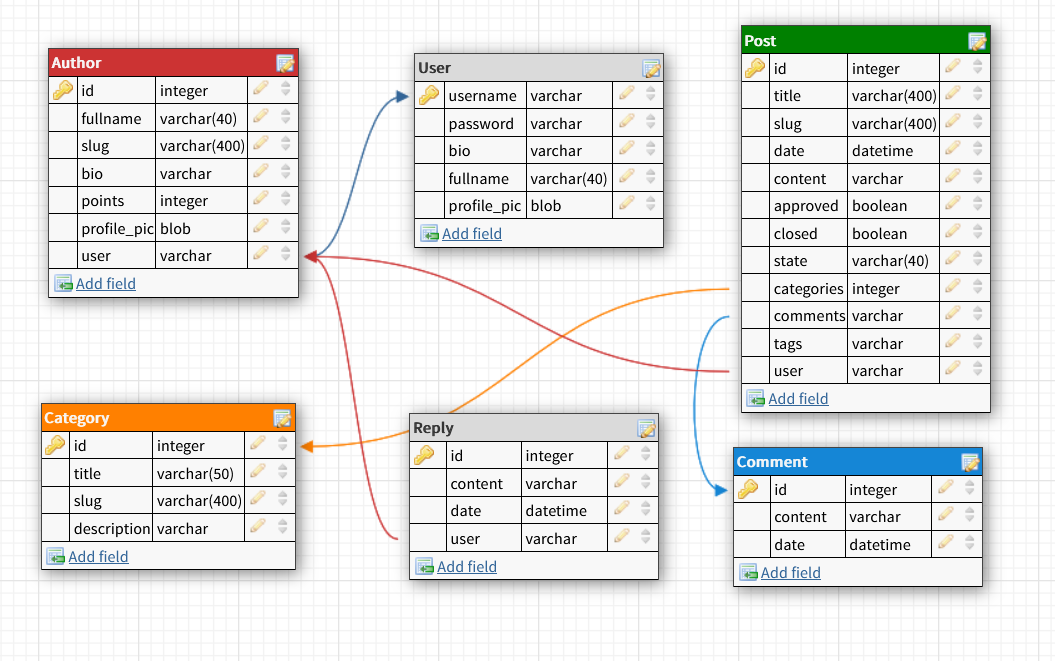
\includegraphics[width=\linewidth]{database}
	\caption{Schema diagram of the database for community forum.}
	\label{fig:8}
\end{figure}

\def\baselinestretch{1.66}
\medskip

%%% ----------------------------------------------------------------------
